
\documentclass[11pt,journal]{IEEEtran}


\usepackage{cite}
\usepackage[pdftex]{graphicx}
\usepackage[tight,footnotesize]{subfigure}
\usepackage{float}
\usepackage{fixltx2e}
\usepackage{url}

% correct bad hyphenation here
\hyphenation{op-tical net-works semi-conduc-tor}


\begin{document}

\title{CSE 471 Project Writeup \\ Team Name}

\author{\IEEEauthorblockN{David Ganey, Kerry Martin, Evan Stoll, Michael Theut, and Ben Roos\\}
\IEEEauthorblockA{School of Computing, Informatics and\\Decision Systems Engineering\\
Arizona State University\\
CSE 471\\}
}

% make the title area
\maketitle

\renewcommand{\abstractname}{Executive Summary}
\begin{abstract}
TODO -- this executive summary should take up the entire page
\end{abstract}

\IEEEpeerreviewmaketitle

\section{Part 1}
\section{Part 2}
Part 2 of the project describes another task given by the CEO of the CactusCard Credit Company, wherein a program should be developed to provide ``a \emph{machine learning based approach} to identify individuals who should/should not be given the CactusCardPlus.'' This section will formulate this problem and describe the steps taken to solve it.

\subsection{Problem Formulation}
The problem itself is a machine-learning problem, which at its core simply means a program designed to recognize patterns. Machine learning can encompass a wide variety of problems, which can be divided into ``regression'' problems and ``classification'' problems. In this case, the consumer research division has given the team a dataset which contains information about customers \emph{for whom the decision to award or not to award the CactusCard has already been made}. This is important information -- because customers can either be given the card or not (a binary \emph{classification}), this falls under the realm of ``classification'' machine learning problems. Additionally, the fact that the classification program will be trained with data means this is a ``supervised'' learning problem.
\par
As a supervised classification machine, the program must be able to read the data set and, with that information, draw conclusions about which credit variables have the largest impact on whether or not the customer was given the card. To be an effective tool for the CactusCard corporation, the dataset supplied by the consumer research division should only include proper decisions -- cases where the card was awarded to the correct individual and denied to individuals who would have abused the line of credit. Otherwise, the machine will learn ``bad habits'' and will draw conclusions from the data which are not useful to the company.
\par
The dataset itself is comprised of 15 credit attributes for the individuals, as well as an indication of whether the individual received a card. The credit attributes are not specified, though the problem specification does include the datatypes for each attribute. (For example, attribute 1 can be either ``b'' or ``a'', and therefore represents some binary information about the customer such as whether they are male or female).
\par
The goal of this component of the project is to demonstrate a program which can use the dataset to learn how the credit attributes affect the decision to award the card, and from there use that knowledge to predict card decisions within a certain degree of accuracy.

\subsection{Solution Proposals}
Weka, a software tool developed at the University of Waikato, is a software package with implementations of a large number of machine learning algorithms. Weka can be used in multiple ways. One option is to simply use the Weka API to access the algorithms from Java code. This is advantageous when one wishes to write a full machine learning system. Another option is to use the Weka Explorer, which is a wrapper around the algorithms. This GUI tool allows the user to load a data set and run the algorithms on it, then view the results in various formats.
\par
It is this method which is proposed to solve the task given by the CEO. Using the Weka Explorer, we have a straightforward method for gaining insight into the effect of the 15 credit attributes. We can use the Explorer to test various machine learning algorithms, and based on their success rates, determine which should be used in the future to make the actual issue decision.

\begin{figure}[H]
\centering
    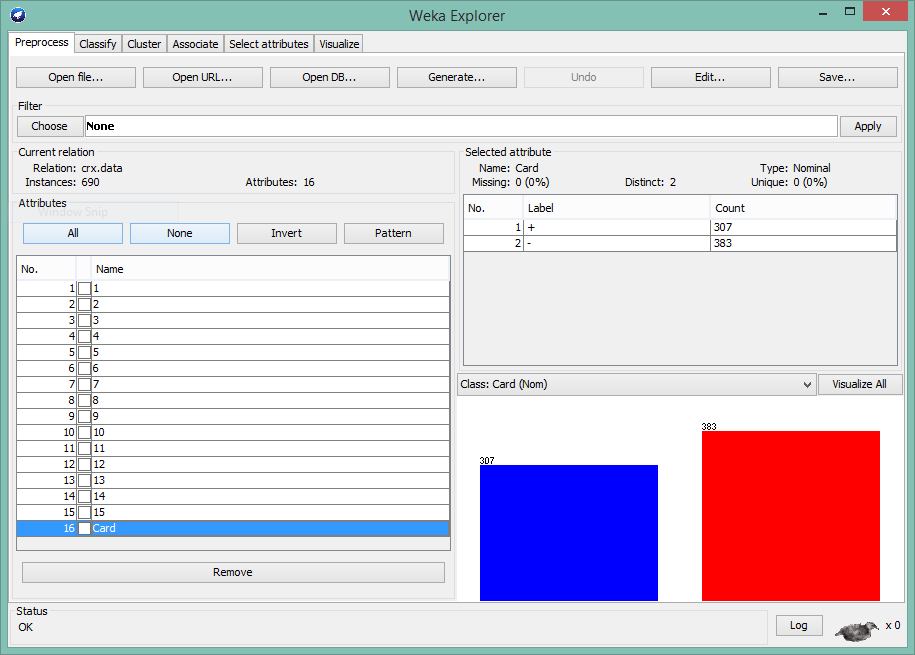
\includegraphics[width=3in]{images/wekaexplorer}
\caption{The Weka Explorer interface}
\label{wekaexplorer}
\end{figure}

\subsection{Test Plan} \label{testplan}
The team will evaluate several popular machine learning algorithms in the Weka Explorer. The success of each algorithm will be determined by a number of factors. The team must consider runtime, as the algorithm cannot take an extreme amount of time to complete or it will be useless. The most important factor, however, is the accuracy of the classification. Using random chance to classify card issuance would theoretically have an accuracy rate of approximately 50\%, so the team must find an algorithm with a higher percentage than that. To ensure CactusCard's continued financial success, the algorithm must predict card issuance correctly at least 80\% of the time.

\subsection{Solution 1}
Support Vector Machines (SVM) are, according to Russell and Norvig, ``the most popular approach for `off-she-shelf' supervised learning''' \cite{ai}. SVMs do a good job of classification because they separate groups as much as possible (called a ``maximum margin separator''). Additionally, SVMs can work in multiple dimensions (creating a ``hyperplane'') which will be important with the high number of credit attributes in the data set. Finally, SVMs are considered a nonparametric method, because they store some of the training examples, and yet like parametric models, they often avoid overfitting the data \cite{ai}.
\par
To use an SVM on the data set provided by the CEO, Weka supports the addition of a library called libsvm. This Java library contains an implementation of the SVM algorithm which hooks into the Weka Explorer interface. The team will set the Explorer to use varying numbers of crossfold validation passes, in order to evaluate the classifier. This will split the dataset, train the SVM with a subset of the dataset, and then evaluate the SVM's effectiveness at predicting the card issuance decision by comparing the SVM's predictions to the actual data. The results from running the libsvm algorithm on the dataset are shown in the table below:

\begin{table}[H]
{\renewcommand{\arraystretch}{1.2}%
\begin{tabular}{|l|l|l|l|}
\hline
Crossfold validations         & 5             & 10            & 15            \\ \hline
Time taken to build model (s) & .19           & .24           & .19           \\ \hline
Correctly classified (\%)     & 382 (55.36\%) & 385 (55.80\%) & 384 (55.65\%) \\ \hline
Incorrectly classified (\%)   & 308 (44.64\%) & 305 (44.20\%) & 306 (44.35\%) \\ \hline
\end{tabular}} \quad
\caption{A table showing the results of the libsvm applied to the data set}
\end{table}

As we can see from the table, no significant difference exists when adjusting the number of crossfold validation passes. All of the attempts fall well within the expected runtime, and predict with approximately 55\% accuracy whether someone was or was not given a CactusCard. While this is consistently better than randomly guessing, it only exceeds that percentage by approximately 5\%. While SVMs are good classifiers, in this instance this algorithm is not a suitable choice for the company, as it fails the criteria established in Section \ref{testplan}.

\subsection{Solution 2}
Another type of machine learning algorithm is called a ``multilayer perceptron.'' This is a type of neural network, which maps from inputs (in this case, the credit attributes) to outputs (whether someone was given a card). The MLP is suitable for this task because it uses ``backpropagation,'' which is a supervised learning technique. 
\par
The multilayer perceptron is significantly more complex than the SVM, but Weka does include an implementation in the Explorer. Using the same technique as above, the team will evaluate this algorithm with various levels of crossfold validation to determine the optimal setting. The results are seen below:

\begin{table}[H]
{\renewcommand{\arraystretch}{1.2}%
	\begin{tabular}{|l|l|l|l|}
\hline
Crossfold validations         & 5             & 10            & 15            \\ \hline
Time taken to build model (s) & 8.46          & 8.47          & 8.51          \\ \hline
Correctly classified (\%)     & 584 (84.64\%) & 572 (82.90\%) & 572 (82.90\%) \\ \hline
Incorrectly classified (\%)   & 106 (15.36\%) & 118 (17.10\%) &           118 (17.10\%)  \\ \hline
\end{tabular}
} \quad
\caption{A table showing the results of the multilayer perceptron applied to the data set}
\end{table}

Once again, it is clear that adjusting the number of crossfold validations has little to no effect on the accuracy of the classifier. As a result, the recommendation of the team is to use 5 validations on data sets of this size, so the algorithm does not take too long to run. While the time taken to build the data model was always nearly the same, the total runtime for all passes of the validation increased dramatically at 15 validations.
\par
Despite the lack of variability among the validation numbers, we can see immediately that the multilayer perceptron is a good choice for the CactusCard company. In all cases, the success of the classifier was above the criteria set above in Section \ref{testplan}. The MLP algorithm averaged approximately 83\% correctness, which is significantly higher than random chance. This algorithm would be a good choice for future data sets, where it could use the information it learned from this training set to choose who receives a card.

% An example of a double column floating figure using two subfigures.
% (The subfig.sty package must be loaded for this to work.)
% The subfigure \label commands are set within each subfloat command, the
% \label for the overall figure must come after \caption.
% \hfil must be used as a separator to get equal spacing.
% The subfigure.sty package works much the same way, except \subfigure is
% used instead of \subfloat.
%
%\begin{figure*}[!t]
%\centerline{\subfloat[Case I]\includegraphics[width=2.5in]{subfigcase1}%
%\label{fig_first_case}}
%\hfil
%\subfloat[Case II]{\includegraphics[width=2.5in]{subfigcase2}%
%\label{fig_second_case}}}
%\caption{Simulation results}
%\label{fig_sim}
%\end{figure*}
%
% Note that often IEEE papers with subfigures do not employ subfigure
% captions (using the optional argument to \subfloat), but instead will
% reference/describe all of them (a), (b), etc., within the main caption.

\section{Conclusion}
The conclusion goes here.




% conference papers do not normally have an appendix


% use section* for acknowledgement
\section*{Acknowledgment}


The authors would like to thank...





% trigger a \newpage just before the given reference
% number - used to balance the columns on the last page
% adjust value as needed - may need to be readjusted if
% the document is modified later
%\IEEEtriggeratref{8}
% The "triggered" command can be changed if desired:
%\IEEEtriggercmd{\enlargethispage{-5in}}

% references section

% can use a bibliography generated by BibTeX as a .bbl file
% BibTeX documentation can be easily obtained at:
% http://www.ctan.org/tex-archive/biblio/bibtex/contrib/doc/
% The IEEEtran BibTeX style support page is at:
% http://www.michaelshell.org/tex/ieeetran/bibtex/
%\bibliographystyle{IEEEtran}
% argument is your BibTeX string definitions and bibliography database(s)
%\bibliography{IEEEabrv,../bib/paper}
%
% <OR> manually copy in the resultant .bbl file
% set second argument of \begin to the number of references
% (used to reserve space for the reference number labels box)
\begin{thebibliography}{1}

\bibitem{IEEEhowto:kopka}
H.~Kopka and P.~W. Daly, \emph{A Guide to \LaTeX}, 3rd~ed.\hskip 1em plus
  0.5em minus 0.4em\relax Harlow, England: Addison-Wesley, 1999.

\end{thebibliography}



% that's all folks
\end{document}


